\newpage
\section{Theory} \label{sec:theory}

To gain an understanding of the motivations behind this project it is worthwhile to discuss both prior work done with the PDH method, and the motivations behind using it to lock to an atomic source.  The PDH method is often used to lock a laser to an actuated cavity \cite{black1998}.  The Madison group primarily performs laser cooling experiments on Lithium and Rubidium gas.  They need to precisely set laser frequencies at or near key atomic transitions. This project focuses on the Rb87 and Rb85 $5S_{1/2} \rightarrow 5P_{3/2}$ transitions, specifically the Rb87 $\left|F=2\right\rangle \rightarrow F'$ and Rb85 $\left|F=3\right\rangle \rightarrow F'$.  The closer a laser's frequency is to a desired transition and the smaller the linewidth of that laser, the more efficient any excitation will be.  This has a direct impact on experimental outcome. \\

Talk about optical phase modulation, PDH. State here again that it is the absorption spectrum resonance features that are to be used for frequency locking.

%%%%%%%%%%%%%%%%%%%%%%%%%%%%%%%%%%%%%%%%%%%%%%%%%%%%%%%%%%%
%%%%%%%%    Phase Modulation
%%%%%%%%%%%%%%%%%%%%%%%%%%%%%%%%%%%%%%%%%%%%%%%%%%%%%%%%%%%

\subsection{Optical Phase Modulation}

As it is not possible to process optical signals in the THz range electronically, it is common to modulate these signals to produce a spectrum about the carrier, and then down-mix them to RF signals to extract the relevant information. For optical signals, this is typically done with either an AOM or an EOM. From a mathematical standpoint, the only difference between the two methods is what phase modulation depths and frequencies are physically attainable. \\

With AOMs, which use acoustic waves to Doppler shift a beam in the transverse direction of propagation, there is a distinct tradeoff between modulation frequency and the resultant power of the outgoing beam.  The AOMs in current use by the Madison Group only have a useful modulation frequency of approximately 200 kHz \cite{madison14}. \\

The modulation frequency of an EOM is sustainable well into the 100 MHz range, with modulation depth a function of the driving voltage. Furthermore, as phase modulation is parallel with the beam propagation, there is no significant decrease in total beam power as the modulation frequency is increased. High modulation frequencies do, however, result in higher electrical power consumption. Typical modulation depths are in the 100mRad range, with a driving voltage of $\sim 10 V_{pp}$ \cite{thorlabs_eom}. A higher modulation depth demands a higher driving voltage, which also results in higher power dissipation. \\

The effect of the phase modulating medium is to induce a phase oscillation in the incident laser:
\begin{gather}
  E = E_0 e^{i\omega t} \xrightarrow{\mbox{Phase Modulation}}
    E_0 e^{i \omega t + \beta \sin \Omega t}
\end{gather}
where $\beta$ is defined as the modulation depth, in radians, and $\Omega$ is the modulation frequency. Using the Jacobi-Anger expansion to isolate the sideband amplitudes,

\begin{gather}
  E_0 e^{i \omega t + \beta \sin \Omega t}  =
  E_0 e^{i\omega t} \sum_{n = -\infty}^{n = \infty} J_n(\beta)e^{in\Omega}
\end{gather}

it is shown that a sideband of frequency $(\omega +n\Omega)$ has amplitude $J_n(\beta)$, the Bessel function of order $n$, evaluated at $\beta$, the modulation depth. If the modulation depth is sufficiently small, the following linear approximation can be made:

\begin{gather}
  E_0 e^{i \omega t + \beta \sin \Omega t}  \approx
    E_0 e^{i\omega t} \left(1 + \frac{\beta}{2}e^{i\Omega t} -
      \frac{\beta}{2} e^{-i\Omega t} \right)
\end{gather}

An inspection of Bessel function behaviour near the origin shows that this approximation quickly becomes invalid for large modulation depths, and that the carrier amplitude is not conserved. This phenomenon becomes important when considering the response of a photosensor to the carrier and side-band amplitudes. These must be tuned such that the signal power is above the noise floor of the FO receiver, but below the saturation level.

% \begin{figure}
%   \centering
%   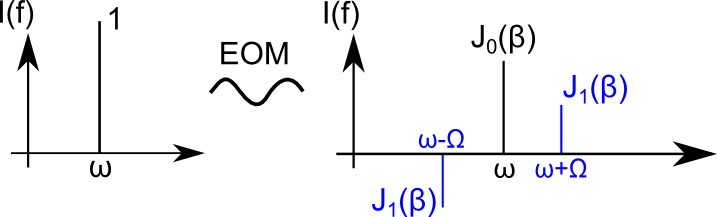
\includegraphics[scale=1.2]{spectrum.pdf}
%   \caption{Expected spectrum of beam after phase modulation, to the first
%   sidebands. While possibly present and significant, further sidebands can
%   be ignored as they will be filtered during mixing.}
%   \label{fig:eom_spectrum}
% \end{figure}

%%%%%%%%%%%%%%%%%%%%%%%%%%%%%%%%%%%%%%%%%%%%%%%%%%%%%%%%%%%
%%%%%%%%   PDH Method
%%%%%%%%%%%%%%%%%%%%%%%%%%%%%%%%%%%%%%%%%%%%%%%%%%%%%%%%%%%

\subsection{The Pound-Drever-Hall Method}

\subsubsection{Fabry-Pi{\'e}rot Cavity Reference}

Makes sense to briefly discuss this and how it is made use of in this project.

Fabry-P{\'e}rot cavity with reflection coefficient $R(\omega)=E_{r}/E_{in}$.
\ggather{
  E_r = E_0\left[R(\omega)e^{i\omega t} + R(\omega+ \Omega)e^{i(\omega + \Omega)t} -
  R(\omega - \Omega)e^{i(\omega - \Omega)t} \right]
}
$R(\omega)$ is complex valued. The voltage and current generated by standard photosensor/transimpedance amplifier unit is proportional to the incident optical power. Adopting the notation $F(\omega) = F, F(\omega \pm \Omega) = F_\pm$, for any frequency selective function F, the following electrical signal is expected:
\ggather{
  \begin{gathered}
    I \propto |E_r|^2 = E_0^2 \left[ |R|^2 + \frac{\beta^2}{4}\left(|R_+|^2 + |R_-|^2\right) + \right.
\\
    \left. \beta(\Re[X(\omega)]\cos\Omega t + \Im[X(\omega)]\sin\Omega t) + \frac{\beta^2}{2}(R_+R_-^\star e^{i2\Omega t} - R_-R_+^\star e^{-i2\Omega t})\right] \\
  \end{gathered} \\
  X(\omega) = R R_+^\star - R^\star R_-
}
after band pass filter in a sufficient bandwidth around $\Omega$ and mixed with a reference VCO with phase offset $\phi$ from the driver and with frequency $\Omega$ (can be derived from driver signal):
\nggather{
  \nonumber V \propto |E_0|^2 \beta(\Re[X(\omega)]\cos\Omega t + \Im[X(\omega)]\sin\Omega t) V_{VCO}\cos(\Omega t + \phi)
}
filtering at some $\omega_f < \Omega$:
\ggather{
  V \propto |E_0|^2 \beta(\Re[X(\omega)]\cos \phi + \Im[X(\omega)]\sin\phi)
}
by adjusting $\phi$ appropriately, one can extract either $(\Re[X(\omega)]$ or $(\Im[X(\omega)]$. Alternatively, by setting up a quadrature demodulation path, with two references $\pi/2$ out of phase, both signals can be accessible in parallel.

\subsubsection{Atomic Gas Reference}

Instead of a reflection from FPC, our beam is changed by it's transmission through an atomic gas. Given a frequency dependent susceptibility $\chi(\omega)$, the complex index of refraction can be defined as \cite{steckoptics}:
\ggather{
  \tilde{n}(\omega) = \sqrt{1 + \chi(\omega)} \\
  n(\omega) = \Re[\tilde{n}(\omega)] \quad \quad a(\omega) \propto \Im[\tilde{n}(\omega)]
}
where $n(\omega)$, $a(\omega)$ are the real index of refraction and absorption, respectively. Using a standard, weakly-intecting, complex susceptibility model for an atomic gas, these are approximately \cite{steckoptics} (see derivations behind (17.25), (17.26)):
\ggather{
  n(\omega) \approx 1 + \frac{N e^2}{2m\epsilon_0}\frac{(\omega_0 - \omega/2\omega)}{(\omega_0-\omega)^2 +(\Gamma/2)^2} \label{eq:n} \\
  a(\omega) \approx \frac{N e^2}{m \epsilon_0 c_0 \Gamma} \frac{(\Gamma/2)^2}{(\omega_0-\omega)^2+(\Gamma/2)^2} \label{eq:a}
}
where $\omega_0$ is a transition resonance and $\Gamma$ is the FWHM (in rad/s) of the absorption feature. These terms are derived from a complex valued function and are related through the Kramers-Kronig relations.\\

As a beam passes through this medium, one can derive a complex valued transmission function, $T(\omega)=\tau(\omega)e^{i\phi_T(\omega)}$,as a function of optical path length, L. After some brief algebraic manipulation:
\ggather{
  \tau(\omega) = e^{-a(\omega)L} \label{eq:tau} \\
  \phi_T(\omega) = (1 - n(\omega)) \frac{\omega}{c} L \label{eq:phit}
}
where $\phi_T(\omega)$ is the \emph{additional} phase accumulation from the presence of the cell. Just like the Fabry-P{\'e}rot cavity, this can be used in a Pound-Drever-Hall system to generate the following electrical signal:
\ggather{
  V \propto |E_0|^2 \beta(\Re[Y(\omega)]\cos\Omega t + \Im[Y(\omega)]\sin\Omega t) \label{eq:v_pdh_gas} \\
  Y(\omega) = TT_+^\star - T^\star T_-
}
and, similarly, through either single channel or quadrature demodulation, this signal can be extracted and used for locking.

%%%%%%%%%%%%%%%%%%%%%%%%%%%%%%%%%%%%%%%%%%%%%%%%%%%%%%%%%%%
%%%%%%%%   Saturated Absorption
%%%%%%%%%%%%%%%%%%%%%%%%%%%%%%%%%%%%%%%%%%%%%%%%%%%%%%%%%%%

\subsection{Saturated Absorption Spectroscopy}

%%%%%%%%%%%%%%%%%%%%%%%%%%%%%%%%%%%%%%%%%%%%%%%%%%%%%%%%%%%
%%%%%%%%   Error Signal Gen
%%%%%%%%%%%%%%%%%%%%%%%%%%%%%%%%%%%%%%%%%%%%%%%%%%%%%%%%%%%

\subsection{Error Signal Generation}

Using the electrical signal in \ref{eq:v_pdh_gas}, single channel demodulation using some $V_{VCO} = v_{vco}\cos(\Omega t+ \phi)$ and then filtering at some $\Omega << \omega_f << 2\Omega$, the resulting DCerror signal is:
\ggather{
  \epsilon \propto \Re[Y(\omega)]\cos\phi + \Im[Y(\omega)]\sin\phi
}
One can select between $\phi = 0, \pi/2$ to extract either the real or imaginary component of $Y(\omega)$. It's worth investigating briefly what the in-phase and quadrature components of $Y(\omega)$ are ( (\ref{eq:pdh_in_phase}) and (\ref{eq:pdh_quadrature}), respectively). Defining $R = r + i\mathbb{R}$:
\ggather{
  \nonumber Y(\omega) = (T + i\mathbb{T})(T_+ - i\mathbb{T}_+) - (T - i\mathbb{T}_+)(T_- + i\mathbb{T}_-) \\
  \Re[Y(\omega)] = T(T_+ - T_-) + \mathbb{T}(\mathbb{T}_+ - \mathbb{T}_-) \label{eq:pdh_in_phase}\\
  \Im[Y(\omega)] = \mathbb{T}(T_- - T_+) + T(\mathbb{T}_+ - \mathbb{T}_-)\label{eq:pdh_quadrature}
}
Note that, both of these signals have zero crossings at the atomic resonances and so their location in frequency space is conserved, which is of obvious use. These signals are shown in \textbf{Figure \ref{fig:pdh_error}} computed for an absorption spectrum about a sample resonance. \\

Alternatively, through quadrature mixing, one can extract both values in separate channels:
\ggather{
  \epsilon_1 = \Re[Y(\omega)]\cos\phi \quad \quad \epsilon_2 = \Im[Y(\omega)]\cos\phi
}
where $\phi=0$ would presumably stay constant to maximize the signals. These separate channels could be used to create a variety of error signals. However, given the response shown in \textbf{Figure \ref{fig:pdh_error}} it is not clear that this is necessary, or even drsirable. For null locking, the in-phase feature defined by (\ref{eq:pdh_in_phase}) is likely sufficient.

\begin{figure}
  \includegraphics[width=0.94\textwidth]{figures/{pdh_error}.png}
  \caption{In-phase and quadrature PDH error signals calculated for a simple model of the Rb85 $\left|F=3\right\rangle \rightarrow \left|F'=3\right\rangle$ resonance using (\ref{eq:n}) (\ref{eq:a}) (\ref{eq:tau}) (\ref{eq:phit}) with $w_0\approx$ 383 THz, $\Gamma \approx$ 5.75 MHz. Note that the in-phase signal has a clear zero crossing at the resonance center, making it ideal for null locking.}
  \label{fig:pdh_error}
\end{figure}

%%%%%%%%%%%%%%%%%%%%%%%%%%%%%%%%%%%%%%%%%%%%%%%%%%%%%%%%%%%
%%%%%%%%   Mod Transfer Spectroscopy
%%%%%%%%%%%%%%%%%%%%%%%%%%%%%%%%%%%%%%%%%%%%%%%%%%%%%%%%%%%

\subsection{Modulation Transfer Spectroscopy}

During development, the saturated absorption signal was difficult to work with, and, given the nature of its probe/pump ratio did not yield signals with very high SNR (see figure). \\

Unlike the saturated absorption signal above, the modulation transfer signal gives slightly different response. At a variety of modulation frequencies in the range of 10-20MHz, both the in-phase and quadrature \cite{0957-0233-19-10-105601}.